\documentclass[a4paper,12pt,twoside]{memoir}

% Castellano
\usepackage[spanish,es-tabla]{babel}
\selectlanguage{spanish}
\usepackage[utf8]{inputenc}
\usepackage[T1]{fontenc}
\usepackage{lmodern} % Scalable font
\usepackage{microtype}
\usepackage{placeins}
\usepackage{float}
\usepackage{adjustbox}
\usepackage{graphicx}



\RequirePackage{booktabs}
\RequirePackage[table]{xcolor}
\RequirePackage{xtab}
\RequirePackage{multirow}

% Links
\PassOptionsToPackage{hyphens}{url}\usepackage[colorlinks]{hyperref}
\hypersetup{
	allcolors = {red}
}

% Ecuaciones
\usepackage{amsmath}

% Rutas de fichero / paquete
\newcommand{\ruta}[1]{{\sffamily #1}}

% Párrafos
\nonzeroparskip

% Huérfanas y viudas
\widowpenalty100000
\clubpenalty100000

% Imágenes

% Comando para insertar una imagen en un lugar concreto.
% Los parámetros son:
% 1 --> Ruta absoluta/relativa de la figura
% 2 --> Texto a pie de figura
% 3 --> Tamaño en tanto por uno relativo al ancho de página
\usepackage{graphicx}
\newcommand{\imagen}[3]{
	\begin{figure}[!h]
		\centering
		\includegraphics[width=#3\textwidth]{#1}
		\caption{#2}\label{fig:#1}
	\end{figure}
	\FloatBarrier
}

% Comando para insertar una imagen sin posición.
% Los parámetros son:
% 1 --> Ruta absoluta/relativa de la figura
% 2 --> Texto a pie de figura
% 3 --> Tamaño en tanto por uno relativo al ancho de página
\newcommand{\imagenflotante}[3]{
	\begin{figure}
		\centering
		\includegraphics[width=#3\textwidth]{#1}
		\caption{#2}\label{fig:#1}
	\end{figure}
}

% El comando \figura nos permite insertar figuras comodamente, y utilizando
% siempre el mismo formato. Los parametros son:
% 1 --> Porcentaje del ancho de página que ocupará la figura (de 0 a 1)
% 2 --> Fichero de la imagen
% 3 --> Texto a pie de imagen
% 4 --> Etiqueta (label) para referencias
% 5 --> Opciones que queramos pasarle al \includegraphics
% 6 --> Opciones de posicionamiento a pasarle a \begin{figure}
	\newcommand{\figuraConPosicion}[6]{%
		\setlength{\anchoFloat}{#1\textwidth}%
		\addtolength{\anchoFloat}{-4\fboxsep}%
		\setlength{\anchoFigura}{\anchoFloat}%
		\begin{figure}[#6]
			\begin{center}%
				\Ovalbox{%
					\begin{minipage}{\anchoFloat}%
						\begin{center}%
							\includegraphics[width=\anchoFigura,#5]{#2}%
							\caption{#3}%
							\label{#4}%
						\end{center}%
					\end{minipage}
				}%
			\end{center}%
		\end{figure}%
	}
	
	%
	% Comando para incluir imágenes en formato apaisado (sin marco).
	\newcommand{\figuraApaisadaSinMarco}[5]{%
		\begin{figure}%
			\begin{center}%
				\includegraphics[angle=90,height=#1\textheight,#5]{#2}%
				\caption{#3}%
				\label{#4}%
			\end{center}%
		\end{figure}%
	}
	% Para las tablas
	\newcommand{\otoprule}{\midrule [\heavyrulewidth]}
	%
	% Nuevo comando para tablas pequeñas (menos de una página).
	\newcommand{\tablaSmall}[5]{%
		\begin{table}
			\begin{center}
				\rowcolors {2}{gray!35}{}
				\begin{tabular}{#2}
					\toprule
					#4
					\otoprule
					#5
					\bottomrule
				\end{tabular}
				\caption{#1}
				\label{tabla:#3}
			\end{center}
		\end{table}
	}
	
	%
	% Nuevo comando para tablas pequeñas (menos de una página).
	\newcommand{\tablaSmallSinColores}[5]{%
		\begin{table}[H]
			\begin{center}
				\begin{tabular}{#2}
					\toprule
					#4
					\otoprule
					#5
					\bottomrule
				\end{tabular}
				\caption{#1}
				\label{tabla:#3}
			\end{center}
		\end{table}
	}
	
	\newcommand{\tablaApaisadaSmall}[5]{%
		\begin{landscape}
			\begin{table}
				\begin{center}
					\rowcolors {2}{gray!35}{}
					\begin{tabular}{#2}
						\toprule
						#4
						\otoprule
						#5
						\bottomrule
					\end{tabular}
					\caption{#1}
					\label{tabla:#3}
				\end{center}
			\end{table}
		\end{landscape}
	}
	
	%
	% Nuevo comando para tablas grandes con cabecera y filas alternas coloreadas en gris.
	\newcommand{\tabla}[6]{%
		\begin{center}
			\tablefirsthead{
				\toprule
				#5
				\otoprule
			}
			\tablehead{
				\multicolumn{#3}{l}{\small\sl continúa desde la página anterior}\\
				\toprule
				#5
				\otoprule
			}
			\tabletail{
				\hline
				\multicolumn{#3}{r}{\small\sl continúa en la página siguiente}\\
			}
			\tablelasttail{
				\hline
			}
			\bottomcaption{#1}
			\rowcolors {2}{gray!35}{}
			\begin{xtabular}{#2}
				#6
				\bottomrule
			\end{xtabular}
			\label{tabla:#4}
		\end{center}
	}
	
	%
	% Nuevo comando para tablas grandes con cabecera.
	\newcommand{\tablaSinColores}[6]{%
		\begin{center}
			\tablefirsthead{
				\toprule
				#5
				\otoprule
			}
			\tablehead{
				\multicolumn{#3}{l}{\small\sl continúa desde la página anterior}\\
				\toprule
				#5
				\otoprule
			}
			\tabletail{
				\hline
				\multicolumn{#3}{r}{\small\sl continúa en la página siguiente}\\
			}
			\tablelasttail{
				\hline
			}
			\bottomcaption{#1}
			\begin{xtabular}{#2}
				#6
				\bottomrule
			\end{xtabular}
			\label{tabla:#4}
		\end{center}
	}
	
	%
	% Nuevo comando para tablas grandes sin cabecera.
	\newcommand{\tablaSinCabecera}[5]{%
		\begin{center}
			\tablefirsthead{
				\toprule
			}
			\tablehead{
				\multicolumn{#3}{l}{\small\sl continúa desde la página anterior}\\
				\hline
			}
			\tabletail{
				\hline
				\multicolumn{#3}{r}{\small\sl continúa en la página siguiente}\\
			}
			\tablelasttail{
				\hline
			}
			\bottomcaption{#1}
			\begin{xtabular}{#2}
				#5
				\bottomrule
			\end{xtabular}
			\label{tabla:#4}
		\end{center}
	}
	
	
	
	\definecolor{cgoLight}{HTML}{EEEEEE}
	\definecolor{cgoExtralight}{HTML}{FFFFFF}
	
	%
	% Nuevo comando para tablas grandes sin cabecera.
	\newcommand{\tablaSinCabeceraConBandas}[5]{%
		\begin{center}
			\tablefirsthead{
				\toprule
			}
			\tablehead{
				\multicolumn{#3}{l}{\small\sl continúa desde la página anterior}\\
				\hline
			}
			\tabletail{
				\hline
				\multicolumn{#3}{r}{\small\sl continúa en la página siguiente}\\
			}
			\tablelasttail{
				\hline
			}
			\bottomcaption{#1}
			\rowcolors[]{1}{cgoExtralight}{cgoLight}
			
			\begin{xtabular}{#2}
				#5
				\bottomrule
			\end{xtabular}
			\label{tabla:#4}
		\end{center}
	}
	
	
	
	\graphicspath{ {./img/} }
	
	% Capítulos
	\chapterstyle{bianchi}
	\newcommand{\capitulo}[2]{
		\setcounter{chapter}{#1}
		\setcounter{section}{0}
		\setcounter{figure}{0}
		\setcounter{table}{0}
		\chapter*{\thechapter.\enskip #2}
		\addcontentsline{toc}{chapter}{\thechapter.\enskip #2}
		\markboth{#2}{#2}
	}
	
	% Apéndices
	\renewcommand{\appendixname}{Apéndice}
	\renewcommand*\cftappendixname{\appendixname}
	
	\newcommand{\apendice}[1]{
		%\renewcommand{\thechapter}{A}
		\chapter{#1}
	}
	
	\renewcommand*\cftappendixname{\appendixname\ }
	
	% Formato de portada
	\makeatletter
	\usepackage{xcolor}
	\newcommand{\tutor}[1]{\def\@tutor{#1}}
	\newcommand{\course}[1]{\def\@course{#1}}
	\definecolor{cpardoBox}{HTML}{E6E6FF}
	\def\maketitle{
		\null
		\thispagestyle{empty}
		% Cabecera ----------------
		\noindent
\includegraphics[width=\textwidth]{cabecera}\vspace{1cm}%
		\vfill
		% Título proyecto y escudo informática ----------------
		\colorbox{cpardoBox}{%
			\begin{minipage}{.8\textwidth}
				\vspace{.5cm}\Large
				\begin{center}
					\textbf{TFG del Grado en Ingeniería Informática}\vspace{.6cm}\\
					\textbf{\LARGE\@title{}}
				\end{center}
				\vspace{.2cm}
			\end{minipage}
			
		}%
		\hfill\begin{minipage}{.20\textwidth}
			
\includegraphics[width=\textwidth]{escudoInfor}
		\end{minipage}
		\vfill
		% Datos de alumno, curso y tutores ------------------
		\begin{center}%
			{%
				\noindent\LARGE
				Presentado por \@author{}\\ 
				en Universidad de Burgos --- \@date{}\\
				Tutor: \@tutor{}\\
			}%
		\end{center}%
		\null
		\cleardoublepage
	}
	\makeatother
	
	\newcommand{\nombre}{Alejandro Villar Solla} %%% cambio de comando
	
	% Datos de portada
	\title{Implementación de una
		Prueba de Concepto (PoC) de
		Manage Engine PAM para la
		Gestión Eficiente de Acceso
		Privilegiado en Organizaciones}
	\author{\nombre}
	\tutor{Luis Antonio Antolín Sánchez}
	\date{\today}
	
	\begin{document}
		
		\maketitle
		
		
		\newpage\null\thispagestyle{empty}\newpage
		
		
		%%%%%%%%%%%%%%%%%%%%%%%%%%%%%%%%%%%%%%%%%%%%%%%%%%%%%%%%%%%%%%%%%%%%%%%%%%%%%%%%%%%%%%%%
		\thispagestyle{empty}
		
		
		\noindent
\includegraphics[width=\textwidth]{cabecera}\vspace{1cm}
		
		\noindent D. Luis Antonio Antolín Sánchez, profesor del Departamento de Ingeniería Informática, área Lenguajes y Sistemas Informáticos.
		
		\noindent Expone:
		
		\noindent Que el alumno D. \nombre, con DNI 35581466Y, ha realizado el Trabajo final de Grado en Ingeniería Informática titulado título de TFG. 
		
		\noindent Y que dicho trabajo ha sido realizado por el alumno bajo la dirección del que suscribe, en virtud de lo cual se autoriza su presentación y defensa.
		
		\begin{center} %\large
			En Burgos, {\large \today}
		\end{center}
		
		\vfill\vfill\vfill
		
		% Author and supervisor
		\begin{minipage}{0.45\textwidth}
			\begin{flushleft} %\large
				Vº. Bº. del Tutor:\\[2cm]
				D. nombre tutor
			\end{flushleft}
		\end{minipage}
		\hfill
		\begin{minipage}{0.45\textwidth}
			\begin{flushleft} %\large
				Vº. Bº. del co-tutor:\\[2cm]
				D. nombre co-tutor
			\end{flushleft}
		\end{minipage}
		\hfill
		
		\vfill
		
		% para casos con solo un tutor comentar lo anterior
		% y descomentar lo siguiente
		%Vº. Bº. del Tutor:\\[2cm]
		%D. nombre tutor
		
		
		\newpage\null\thispagestyle{empty}\newpage
		
		
		
		
		\frontmatter
		
		% Abstract en castellano
		\renewcommand*\abstractname{Resumen}
		\begin{abstract}
			En el presente Trabajo Fin de Grado se aborda la implementación de una Prueba de Concepto (POC) de la solución PAM360 para la gestión de accesos privilegiados en la empresa NTT Data. La gestión de accesos privilegiados es una necesidad crítica en las organizaciones modernas, dado el creciente número de ciberamenazas y la importancia de proteger la información sensible.
			
			La solución PAM360, desarrollada por ManageEngine, ofrece un conjunto completo de herramientas para administrar y asegurar los accesos privilegiados, garantizando que sólo las personas autorizadas puedan acceder a los recursos críticos de la empresa. Este proyecto se ha llevado a cabo en el contexto de NTT Data, una empresa líder en servicios de consultoría y tecnología, con el objetivo de mejorar su seguridad informática y cumplir con los estándares más exigentes de la industria.
			
			Este proyecto no solo contribuye a fortalecer la seguridad de NTT Data, sino que también ofrece una guía práctica y detallada sobre cómo implementar soluciones de gestión de accesos privilegiados en organizaciones de gran envergadura.

		\end{abstract}
		
		\renewcommand*\abstractname{Descriptores}
		\begin{abstract}
			PAM360, ciberseguridad, gestión de accesos, prueba de concepto (POC), control de privilegios, compilance, Privileged Access Management...
			\ldots
		\end{abstract}
		
		\clearpage
		
		% Abstract en inglés
		\renewcommand*\abstractname{Abstract}
		\begin{abstract}
			This Final Degree Project addresses the implementation of a Proof of Concept (POC) of the PAM360 solution for privileged access management in the company NTT Data. Privileged access management is a critical necessity in modern organizations, given the growing number of cyber threats and the importance of protecting sensitive information.
			
			The PAM360 solution, developed by ManageEngine, offers a comprehensive set of tools to manage and secure privileged access, ensuring that only authorized individuals can access business-critical resources. This project has been carried out in the context of NTT Data, a leading consulting and technology services company, with the aim of improving its IT security and complying with the most demanding standards in the industry.
			
			This project not only contributes to strengthening NTT Data's security, but also provides practical and detailed guidance on how to implement privileged access management solutions in large organizations.
		\end{abstract}
		
		\renewcommand*\abstractname{Keywords}
		\begin{abstract}
			PAM360, cybersecurity, access management, proof of concept (POC), privilege control, compilation, Privileged Access Management...
		\end{abstract}

\clearpage

% Indices
\tableofcontents

\clearpage

\listoffigures

\clearpage

\listoftables
\clearpage

\mainmatter
\capitulo{1}{Introducción}

Descripción del contenido del trabajo y de la estructura de la memoria y del resto de materiales entregados.

\section{Contexto y motivación}
Hoy en día, la seguridad informática y la gestión de accesos son dos áreas principales que no deben ser subestimadas en una organización, especialmente si se trata de organizaciones que procesan información delicada y requieren la seguridad de la integridad de sus sistemas. NTT Data es una consultoría con una parte de ciberseguridad muy reconocida que se enfrenta al desafío de gestionar sus accesos de una manera segura y eficiente, ya sea de parte de sus empleados u otros clientes externos.

El alto grado de rotación y la necesidad de permitir accesos de manera temporal complican aún más este desafío.

En este contexto, PAM360~\cite{manageengine2023pam360} es una solución de Gestión de Acceso Privilegiado de extremo a extremo que proporciona un control seguro centralizado de todo el acceso a los recursos empresariales críticos. Ayuda a rastrear todos los movimientos y cambios realizados para la seguridad de un usuario.

He elegido esta tarea que he tenido que realizar en NTT Data porque estoy muy interesado en el área de ciberseguridad. Me gustaría trabajar como pentester\footnote{Un pentester es un profesional que realiza pruebas de penetración para identificar y solucionar vulnerabilidades en sistemas de seguridad.} en mi futuro laboral, así que creo que es una gran oportunidad para aprender nuevas tecnologías de seguridad informática observando su desarrollo desde dentro.




\section{Justificación del Proyecto}
La elección de este proyecto es una decisión consensuada con mi tutor en NTT Data, con la sugerencia de implementar una POC para la solución PAM360 en términos de alta seguridad y efectividad en la administración de accesos, ya que la consultora requiere, con sus múltiples clientes y proyectos, un sistema fuerte que soporte la administración de accesos sin comprometer la seguridad.

PAM360 es una solución que puede gestionar y monitorizar los accesos en tiempo real, lo cual es una mejora con respecto a la característica que tenía anteriormente, mediante la cual se solían inscribir a numerosos usuarios dentro del AD de la empresa y estar pendiente de cuándo se expiran cuentas, de los accesos inapropiados, de los cambios de sudoers en linux, etc.

Esta iniciativa está justificada por los beneficios esperados de la implementación de PAM360, que incluyen:
\begin{itemize}
\item Mejora en la seguridad: Al permitir un mejor control y monitoreo de los accesos, se minimiza el riesgo de accesos no autorizados y se garantiza la integridad de los sistemas de la organización.

\item Eficiencia en la gestión de accesos: La centralización de la gestión de accesos permite una administración más sencilla y eficiente, reduciendo la carga de trabajo del equipo de respuesta y prevención.

\item Flexibilidad y escalabilidad: PAM360 permite adaptarse a las necesidades cambiantes de la empresa, facilitando la gestión de usuarios temporales y externos. En caso de que el usuario necesite privilegios adicionales en cualquier sistema, se pueden asignar directamente desde la misma solución en un ambiente controlado. Se pueden asignar o revocar accesos en cualquier momento.

\end{itemize}

\section{Metodología}

Para la realización de este proyecto, se seguirán los siguientes pasos metodológicos:

\begin{itemize}
\item Revisión de documentación: Investigación y revisión de la documentación técnica relacionada con el tema de gestión de acceso privilegiado y PAM360, por ejemplo, los manuales de ManageEngine y las experiencias de los usuarios

\item Planificación y preparación: Establecimiento del alcance del plan de pruebas, preparación y configuración del entorno de pruebas.

\item Implementación: Despliegue y configuración de PAM360, integración con AD y realización de pruebas funcionales y de seguridad.

\item Evaluación y análisis: Análisis de los resultados, evaluación de la eficacia y efectividad de PAM360.

\item Documentación: Redacción del informe final del proyecto, incluyendo la descripción del proceso, resultados obtenidos,capturas, reportes, conclusiones y recomendaciones.

\end{itemize}

\section{Estructura}
Este documento está organizado de la siguiente manera:

\begin{itemize}
\item Introducción: Presenta el contexto, la justificación, los objetivos, la metodología y la estructura del documento.

\item Objetivos del Proyecto: Detalla los objetivos específicos y generales del proyecto.

\item Conceptos Teóricos: Explica los conceptos teóricos necesarios para entender la gestión de accesos privilegiados y la tecnología subyacente en PAM360.

      \item Secciones: Desglosa las diferentes partes del tema.
      \item Referencias: Lista las fuentes y material consultado.
      \item Imágenes: Presenta diagramas y capturas relevantes.
      \item Listas de ítems: Enumera elementos clave y funcionalidades.
      \item Tablas: Ofrece tablas de datos y comparativas.  
\item Técnicas y Herramientas: Describe las técnicas y herramientas utilizadas durante la implementación y pruebas de PAM360.
\item Aspectos Relevantes del Desarrollo del Proyecto: Aborda los desafíos y consideraciones importantes encontrados durante la configuración y pruebas de PAM360.
\item Trabajos Relacionados: Revisa otros trabajos y estudios similares para situar el proyecto en un contexto más amplio.
\item Conclusiones y Líneas de Trabajo Futuras: Presenta las conclusiones del proyecto y sugiere posibles líneas de trabajo futuras para mejorar y expandir la implementación de PAM360 en NTT Data.
\item Anexos: Incluyen el resto de información que no se ha podido incluir en esta memoria
\end{itemize}
\capitulo{2}{Objetivos del Proyecto}

El desarrollo de este proyecto tiene como propósito principal implementar y evaluar una Prueba de Concepto (POC) de la solución PAM360 en la infraestructura de NTT Data. Para lograr este propósito, se establecen varios objetivos específicos que abarcan tanto los requisitos funcionales del software como los objetivos técnicos necesarios para llevar a cabo el proyecto de manera satisfactoria. A continuación, se detallan estos objetivos:

\section{Objetivos Funcionales}

\begin{itemize}
	\item \textbf{Despliegue de PAM360:}
	\begin{itemize}
		\item Configurar y desplegar PAM360 en una máquina proporcionada por NTT Data, asegurando que funcione correctamente y esté bien integrada dentro de los parámetros de seguridad de la empresa.
	\end{itemize}
	
	\item \textbf{Gestión de Accesos:}
	\begin{itemize}
		\item Implementar la funcionalidad de PAM360 para gestionar los accesos a las máquinas por parte de los usuarios del Active Directory (AD), tanto internos como clientes, asegurando que todos los accesos sean monitoreados y controlados.
	\end{itemize}
	
	\item \textbf{Seguridad y Control:}
	\begin{itemize}
		\item Asegurar que PAM360 proporcione un control estricto y seguro de los accesos, minimizando el riesgo de accesos no autorizados y mejorando la seguridad interna de la infraestructura de NTT Data.
	\end{itemize}
\end{itemize}

\section{Objetivos Técnicos}

\begin{itemize}
	\item \textbf{Integración con Active Directory:}
	\begin{itemize}
		\item Integrar PAM360 con el sistema de Active Directory (AD) de NTT Data para centralizar la gestión de accesos y facilitar la administración de usuarios.
	\end{itemize}
	
	\item \textbf{Configuración y Personalización:}
	\begin{itemize}
		\item Realizar la configuración inicial de PAM360, ajustando los parámetros y opciones para que se adapten a las necesidades específicas de la empresa y aseguren un funcionamiento óptimo.
	\end{itemize}
	
	\item \textbf{Pruebas de Funcionamiento y Seguridad:}
	\begin{itemize}
		\item Llevar a cabo una serie de pruebas funcionales y de seguridad para verificar que PAM360 opera correctamente, identificando y resolviendo cualquier problema que pueda surgir durante el proceso.
	\end{itemize}
	
	\item \textbf{Documentación del Proceso:}
	\begin{itemize}
		\item Documentar detalladamente cada fase del proyecto, desde la configuración y despliegue hasta las pruebas y resultados, recopilando todos los datos al finalizar.
	\end{itemize}
	
	\item \textbf{Evaluación de Resultados:}
	\begin{itemize}
		\item Evaluar el rendimiento y la efectividad de PAM360 en la gestión de accesos y la mejora de la seguridad, recopilando datos y métricas que permitan analizar su funcionamiento.
	\end{itemize}
\end{itemize}

\section{Objetivos de Mejora y Futuro}

\begin{itemize}
	\item \textbf{Optimización Continua:}
	\begin{itemize}
		\item Identificar posibles mejoras en la configuración y uso de PAM360 para optimizar su rendimiento y adaptabilidad a futuros proyectos que se oferten en la empresa.
	\end{itemize}
	
	\item \textbf{Capacitación y Transferencia de Conocimiento:}
	\begin{itemize}
		\item Asegurar que el equipo de TI de NTT Data esté capacitado para utilizar y mantener PAM360, proporcionando la formación necesaria y transfiriendo el conocimiento adquirido durante el proyecto.
	\end{itemize}
	
	\item \textbf{Propuestas de Mejora:}
	\begin{itemize}
		\item Sugerir posibles mejoras y nuevas funcionalidades para futuras versiones de PAM360, basadas en la experiencia obtenida durante la POC y el feedback propio.
	\end{itemize}
\end{itemize}

Los objetivos de este proyecto no solo buscan implementar y evaluar la funcionalidad de PAM360, sino también asegurar que la solución se integre de manera eficiente y segura en la infraestructura de NTT Data, proporcionando un control efectivo de los accesos y mejorando la seguridad informática de la empresa.

\capitulo{3}{Conceptos teóricos}

Este proyecto requiere entender varios conceptos teóricos fundamentales relacionados con la gestión de accesos privilegiados y las herramientas utilizadas, los cuales explicaré a continuación.

\section{Gestión de Accesos Privilegiados (PAM)}
La gestión de accesos privilegiados (PAM) es una rama de la ciberseguridad que se centra en controlar y supervisar los accesos de los usuarios con privilegios avanzados a los sistemas críticos de una organización. Estos usuarios privilegiados tienen permisos especiales dados por responsables y en todo momento controlados que les permiten acceder a información sensible, modificar configuraciones del sistema y realizar tareas administrativas. Implementar una solución PAM es esencial para prevenir accesos no autorizados, reducir riesgos de seguridad y cumplir con las normativas (Barrett, 2020)~\cite{barrett2020pam} .

\section{Active Directory (AD)}
Active Directory (AD) es un servicio desarrollado por Microsoft, utilizado en redes de dominio de Windows. Su función principal es gestionar y almacenar información sobre los recursos de la red y los usuarios, permitiendo a los administradores gestionar permisos y controlar el acceso a los recursos de la red de manera centralizada. En este proyecto, AD es fundamental, ya que se integra con PAM360 para gestionar los accesos de los usuarios (Microsoft, 2024)~\cite{microsoft2024ad}.

\section{Prueba de Concepto (POC)}
Una Prueba de Concepto (POC) es una implementación preliminar de una solución destinada a demostrar su viabilidad y efectividad. En este trabajo, la POC se centra en desplegar y configurar PAM360 en un entorno controlado, comprobando que cumple con los requisitos y expectativas de la empresa. Esta etapa es crucial para identificar posibles problemas y asegurar que la solución es adecuada antes de una implementación a mayor escala (Smith, 2019)~\cite{smith2019poc}.

\section{PAM360}
PAM360 es una solución integral de gestión de accesos privilegiados desarrollada por ManageEngine. Ofrece funcionalidades avanzadas para controlar, auditar y monitorear el acceso de usuarios privilegiados a recursos sensibles de la empresa. Sus características principales incluyen la gestión de contraseñas, sesiones privilegiadas, auditoría de accesos y generación de informes. PAM360 destaca por su capacidad de integración con diversas plataformas y su facilidad de uso (ManageEngine, 2023)~\cite{manageengine2023pam360}.

\section{Seguridad de la Información}
La seguridad de la información es una disciplina que se ocupa de proteger la información contra accesos no autorizados, modificaciones indebidas y destrucción. Incluye principios fundamentales como la confidencialidad, integridad y disponibilidad. Implementar una solución PAM contribuye correctamente a la seguridad de la información al garantizar que solo los usuarios autorizados puedan acceder a sistemas y datos críticos (Whitman and Mattord, 2022)~\cite{whitman2022security}.

\section{Zero Trust}

El modelo de seguridad Zero Trust se basa en el principio de que las amenazas pueden provenir tanto del interior como del exterior de la red. En lugar de asumir que las entidades dentro de la red son de confianza, Zero Trust requiere verificación continua de identidad y contexto para otorgar acceso. PAM360 facilita la implementación de este modelo al gestionar y supervisar los accesos privilegiados de manera estricta (Kindervag, 2010)~\cite{kindervag2010zero}.

\section{Integración de Sistemas}

La integración de soluciones PAM con otros sistemas de TI, como SIEM (Security Information and Event Management), IAM (Identity and Access Management), y herramientas de monitoreo, es crucial para una gestión de seguridad efectiva. Esta integración permite una visión holística de la seguridad y facilita la detección y respuesta a incidentes (Johnson, 2018)~\cite{johnson2018integration}.

\section{Auditoría y Monitoreo de Seguridad}

La auditoría y el monitoreo continuo son componentes esenciales de una estrategia de ciberseguridad. Registrar y analizar las acciones de los usuarios privilegiados permite detectar actividades sospechosas y responder a incidentes de manera oportuna. PAM360 ofrece capacidades avanzadas de auditoría y generación de informes, proporcionando visibilidad completa sobre el uso de accesos privilegiados (Moore, 2021)~\cite{moore2021monitoring}.

Este apartado ha sintetizado los conceptos teóricos necesarios para comprender el desarrollo del proyecto. La correcta comprensión e implementación de estos conceptos es fundamental para el éxito de la gestión de accesos privilegiados en cualquier organización.
\capitulo{4}{Técnicas y herramientas}


\section{Metodologías}

Para llevar a cabo este proyecto, se utilizó la metodología de diagrama de Gantt~\cite{gantt}. Esta metodología es  utilizada en la empresa NTT Data en todos los proyectos, y se aplicó de igual manera en la prueba de concepto (POC) de PAM360. La elección de esta metodología se basó en su eficacia para la gestión del tiempo y las tareas, permitiendo una planificación y seguimiento detallado del proyecto. Al utilizar el diagrama de Gantt, se logró una clara visualización de las distintas fases del proyecto, facilitando la identificación de dependencias y el cumplimiento de los plazos establecidos.

\section{Herramientas de desarrollo}

En el desarrollo del proyecto se emplearon diversas herramientas, cada una seleccionada por su idoneidad para las tareas específicas:

\begin{itemize}
	\item \textbf{mRemote}~\cite{mremoteng}: Se utilizó para conectarse al servidor de PAM. Esta herramienta permite gestionar múltiples conexiones de manera eficiente, lo cual fue crucial para acceder y configurar el servidor de PAM360.
	\item \textbf{Habilitación de puertos}: Se habilitó el puerto 8282 para permitir la conexión desde el PC de la empresa al servidor de PAM. Esta configuración fue esencial para asegurar la comunicación entre los sistemas.
	\item \textbf{Windows}: El sistema operativo utilizado para el servidor de PAM y para las operaciones de configuración.
	\item \textbf{Chrome}: Utilizado para acceder a la interfaz web de PAM360, facilitando la administración y configuración del software.
	\item \textbf{Firewall Fortinet}~\cite{fortinet}: Firewall de NTT Data, necesario para conceder permisos de conexión a la máquina de PAM
\end{itemize}

La elección de estas herramientas se basó en su eficacia para la realización las tareas y en las pautas establecidas por la empresa.

\section{Tecnologías y bibliotecas}

En este proyecto, no se utilizaron lenguajes de programación, frameworks o bibliotecas específicos, dado que el enfoque principal fue la configuración y despliegue de PAM360, en lugar del desarrollo de software. 

\section{Comparativas y justificaciones}

Durante la fase inicial del proyecto, se realizaron comparativas entre distintas soluciones de gestión de accesos privilegiados (PAM). Algunas de las soluciones evaluadas incluyeron:

\begin{itemize}
	\item \textbf{CyberArk}~\cite{cyberark}: Conocida por su robustez y funcionalidades avanzadas en la gestión de accesos privilegiados.
	\item \textbf{BeyondTrust}~\cite{beyondtrust}: Reconocida por su enfoque en la seguridad y la gestión de vulnerabilidades.
	\item \textbf{ManageEngine PAM360}: La solución finalmente elegida, destacada por su integración con otros productos de ManageEngine y su relación contractual con NTT Data.
\end{itemize}
	\label{PAM analizados}
\begin{table}[H]
	\centering
	\begin{adjustbox}{max width=\textwidth}
		\begin{tabular}{|l|c|c|c|}
			\hline
			\textbf{Características}                & \textbf{PAM360} & \textbf{BeyondTrust} & \textbf{CyberArk} \\ \hline
			\textbf{Funcionalidades Principales}    & Control de accesos, gestión de contraseñas, auditorías detalladas & Control de accesos, gestión de contraseñas, auditorías detalladas & Control de accesos, gestión de contraseñas, auditorías detalladas \\ \hline
			\textbf{Integración con AD}             & Sí & Sí & Sí \\ \hline
			\textbf{Compatibilidad de Sistemas}     & Windows, Linux, macOS & Windows, Linux, macOS & Windows, Linux, macOS \\ \hline
			\textbf{Implementación}                 & On-premises y Cloud & On-premises y Cloud & On-premises y Cloud \\ \hline
			\textbf{Escalabilidad}                  & Alta & Alta & Alta \\ \hline
			\textbf{Facilidad de Uso}               & Alta & Media & Media \\ \hline
			\textbf{Soporte y Actualizaciones}      & Regular, con opción a soporte premium & Regular, con opción a soporte premium & Regular, con opción a soporte premium \\ \hline
			\textbf{Seguridad y Cumplimiento}       & Cumplimiento de normativas estándar & Cumplimiento de normativas estándar & Cumplimiento de normativas estándar \\ \hline
			\textbf{Costo}                          & Relativamente bajo & Medio-alto & Alto \\ \hline
			\textbf{Características Adicionales}    & Integración con otras soluciones de ManageEngine & Integración con otras soluciones de BeyondTrust & Integración con otras soluciones de CyberArk \\ \hline
		\end{tabular}
	\end{adjustbox}
	\caption{Comparación de PAM360 vs BeyondTrust vs CyberArk}
	\label{tab:comparison}
\end{table}
	
El criterio principal para la selección de PAM360 fue el acuerdo existente entre ManageEngine y NTT Data sobre las cesión de licencias, que facilitó la implementación y soporte de la solución dentro de la empresa. Este acuerdo no solo simplificó el proceso de adquisición, sino que también garantizó una mayor compatibilidad e integración con las herramientas ya utilizadas por NTT Data.



\capitulo{5}{Aspectos relevantes del desarrollo del proyecto}

\section{Aspectos relevantes del desarrollo del proyecto}

\section{Planificación del proyecto}
La planificación del proyecto se llevó a cabo utilizando un diagrama de Gantt, que permitió una gestión detallada y estructurada de todas las fases del proyecto. Este diagrama se actualizó regularmente para reflejar el progreso y realizar ajustes según las necesidades. La planificación detallada ayudó a asegurar que todas las tareas fueran completadas a tiempo y dentro del alcance definido.

\begin{figure}[H]
	\centering
	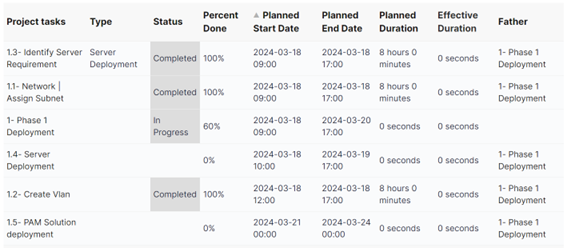
\includegraphics[width=0.8\textwidth]{./img/diagrama1.png}
	\caption{Diagrama del proyecto.}
	\label{fig:diagrama1}
\end{figure}
A continuación, se muestran varias capturas detalladas del diagrama de Gantt, destacando las diferentes fases del proyecto:

\begin{figure}[H]
	\centering
	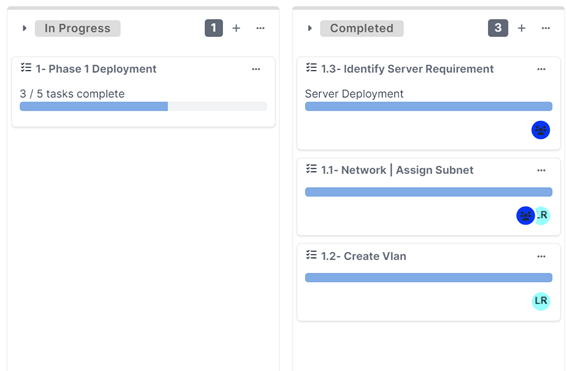
\includegraphics[width=0.8\textwidth]{./img/diagrama2.png}
	\caption{Detalle del diagrama de Gantt.}
	\label{fig:diagrama_detalle1}
\end{figure}

\begin{figure}[H]
	\centering
	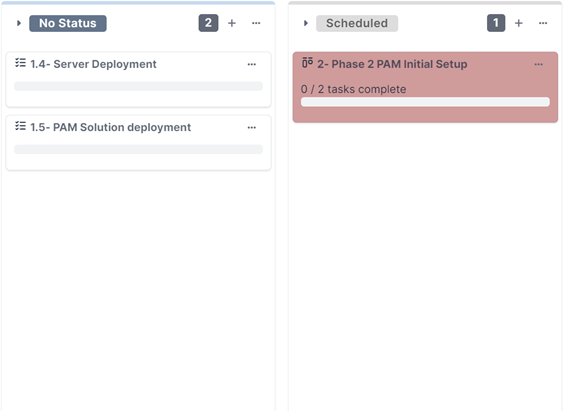
\includegraphics[width=0.8\textwidth]{./img/diagrama3.png}
	\caption{Detalle del diagrama de Gantt: fase de desarrollo.}
	\label{fig:diagrama_detalle2}
\end{figure}


\section{Despliegue de la máquina virtual}
El primer paso del proyecto fue la configuración y despliegue de una máquina virtual en vSphere~\cite{vsphere}. Esta máquina se ha creado con especificaciones adecuadas para soportar PAM360, incluyendo 16 GB de RAM y un sistema operativo Windows Server 2019.

\begin{figure}[H]
	\centering
	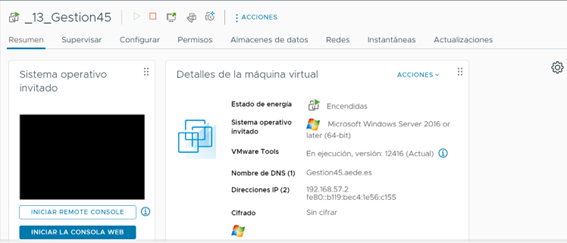
\includegraphics[width=0.8\textwidth]{./img/maquina_pam_vshpere.png}
	\caption{Detalles de la máquina virtual en vSphere.}
	\label{fig:maquina_pam_vshpere}
\end{figure}

\begin{figure}[H]
	\centering
	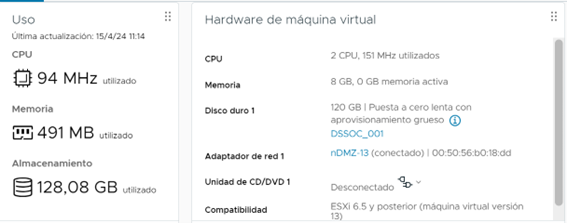
\includegraphics[width=0.8\textwidth]{./img/maquina_pam_detalle.png}
	\caption{Configuración  más detallada de la máquina virtual en vSphere.}
	\label{fig:maquina_pam_vshpere_detalle1}
\end{figure}

\section{Instalación de PAM360}
La instalación de PAM360 se realizó en la máquina virtual utilizando MRemote para la transferencia de archivos y acceso remoto. El proceso de instalación involucró varios pasos, desde la transferencia del archivo ejecutable hasta la configuración inicial del software.

\begin{figure}[H]
	\centering
	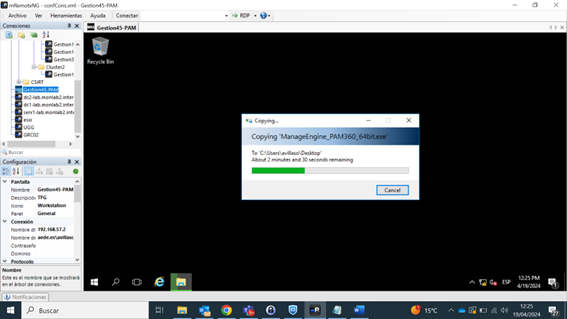
\includegraphics[width=0.8\textwidth]{./img/instalacion_pam.png}
	\caption{Proceso de instalación de PAM360.}
	\label{fig:instalacion_pam}
\end{figure}

\subsection{Proceso de instalación}
El proceso de instalación de PAM360 fue documentado con varias capturas para asegurar la correcta instalación y configuración inicial del software.

\begin{figure}[H]
	\centering
	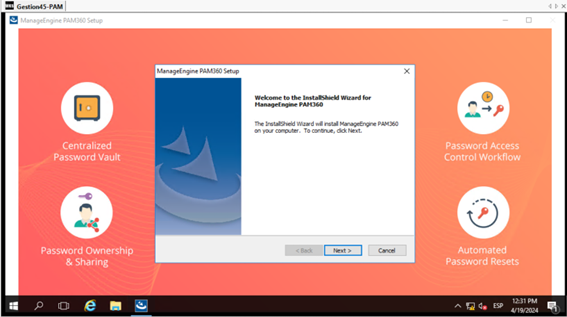
\includegraphics[width=0.8\textwidth]{./img/instalacion_pam2.png}
	\caption{Proceso de instalación de PAM360, primera página.}
	\label{fig:instalacion_detalle1}
\end{figure}

\begin{figure}[H]
	\centering
	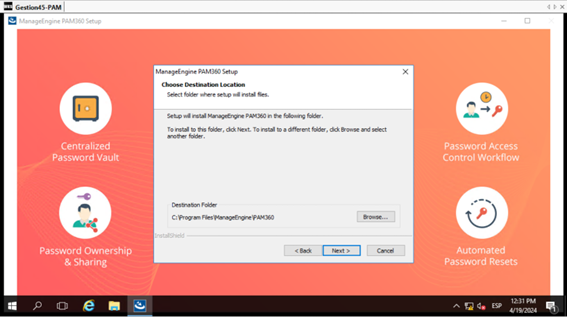
\includegraphics[width=0.8\textwidth]{./img/instalacion_pam3.png}
	\caption{Proceso de instalación de PAM360, segunda página.}
	\label{fig:instalacion_detalle2}
\end{figure}

\begin{figure}[H]
	\centering
	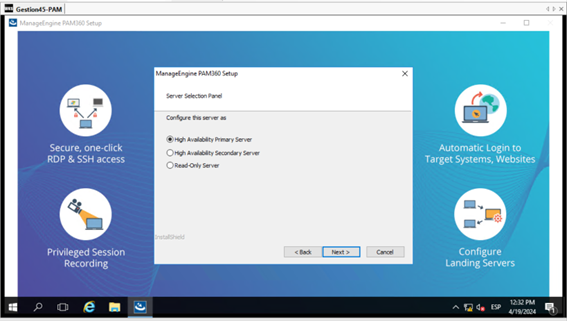
\includegraphics[width=0.8\textwidth]{./img/instalacion_pam4.png}
	\caption{Proceso de instalación de PAM360, tercera y última página.}
	\label{fig:instalacion_detalle3}
\end{figure}

\section{Configuración inicial de PAM360}
Una vez instalado PAM360, se procedió a la configuración inicial, que incluyó el cambio de la contraseña del administrador y la configuración de la autenticación y recursos. Esta fase fue crucial para asegurar que PAM360 estuviera configurado de acuerdo con los requisitos de seguridad de NTT Data.

En las siguientes imágenes se puede observar la aplicación funcionando. 
\begin{figure}[H]
	\centering
	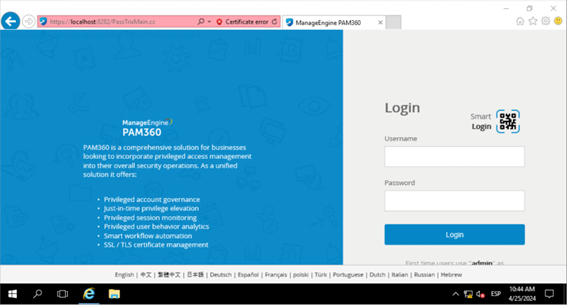
\includegraphics[width=0.8\textwidth]{./img/login_pam_limpio.png}
	\caption{Pantalla principal de PAM.}
	\label{fig:pam_accesoinicial}
\end{figure}


El primer acceso tiene las credenciales por defecto ''admin/admin'' . PAM nos fuerza a que nada más se acceda, se debe cambiar la contraseña por una nueva

\begin{figure}[H]
	\centering
	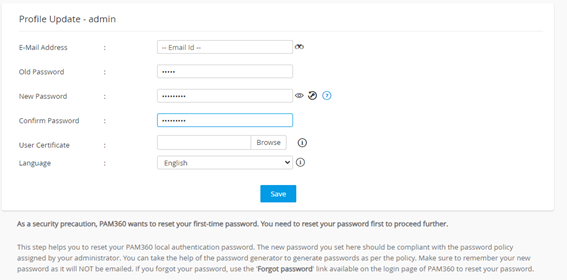
\includegraphics[width=0.8\textwidth]{./img/pam_upadteadmin_pass.png}
	\caption{Configuración del administrador en PAM360.}
	\label{fig:pam_upadteadmin_pass}
\end{figure}

Una vez cambiada, PAM se conectará automáticamente haciéndonos saber que todo ha sido correcto.
\begin{figure}[H]
	\centering
	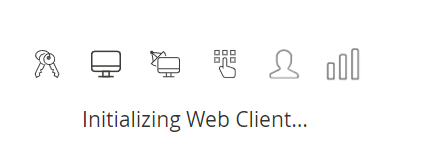
\includegraphics[width=0.8\textwidth]{./img/iniciar_pam.png}
	\caption{Configuración del administrador en PAM360.}
	\label{fig:pam_inicio}
\end{figure}

Dado que no hay ninguna máquina, contraseña o usuario vinculados a la solución, la página podría presentarse de la siguiente manera:

\begin{figure}[H]
	\centering
	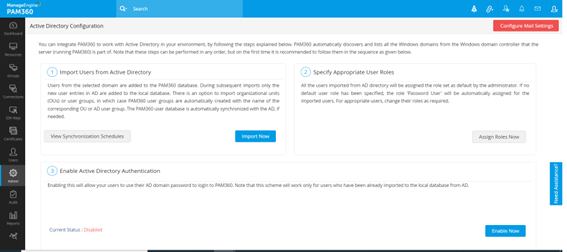
\includegraphics[width=0.8\textwidth]{./img/pam_portada_vanilla.png}
	\caption{Configuración del administrador en PAM360.}
	\label{fig:pam_inicio_limpio}
\end{figure}


\section{Integración con Active Directory}
La integración con Active Directory (AD) fue una de las tareas más importantes del proyecto. Este proceso permitió la importación de usuarios y grupos del AD a PAM360, facilitando el control de acceso y la gestión de credenciales. Se configuró el dominio AD ''NTTDATA'' y se importaron los usuarios necesarios.

\begin{figure}[H]
	\centering
	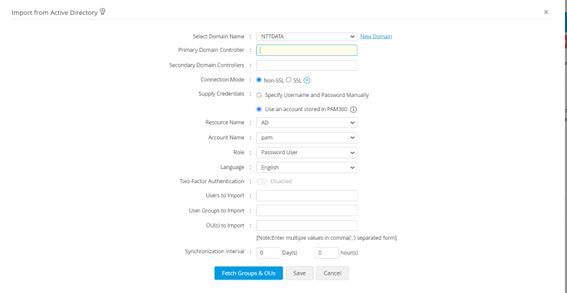
\includegraphics[width=0.8\textwidth]{./img/pam_ad3.png}
	\caption{Importación de usuarios desde Active Directory.}
	\label{fig:pam_ad3}
\end{figure}

Debemos crear una política de password para poder añadir el AD, esto es un requisito adicional de PAM como capa extra de seguridad, para cerciorarse que las contraseñas que pongamos cumplan los requisitos estándar de seguridad.

\begin{figure}[H]
	\centering
	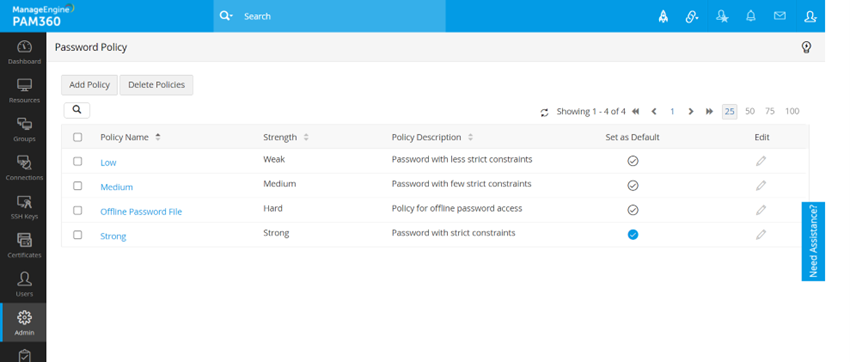
\includegraphics[width=0.8\textwidth]{./img/pam_password_policy.png}
	\caption{Configuración del administrador en PAM360.}
	\label{fig:pam_password_policy}
\end{figure}

Cuando se haya integrado correctamente todo, se debería ver así:

\begin{figure}[H]
	\centering
	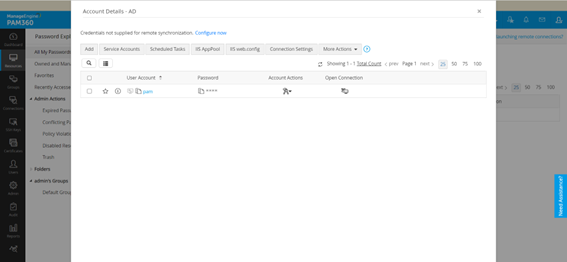
\includegraphics[width=0.8\textwidth]{./img/pam_integradoya_ad.png}
	\caption{AD con la cuenta de pam activo.}
	\label{fig:pam_ad4}
\end{figure}

Una vez creada la entrada para el AD, el siguiente paso era importar los usuarios del AD a los que se vayan a querer dar acceso a las herramientas y así comprobar que la integración con el AD ha sido exitosa.

\begin{figure}[H]
	\centering
	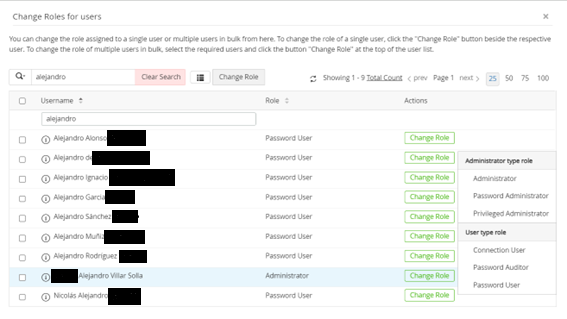
\includegraphics[width=0.8\textwidth]{./img/importacion_usuarios_ad.png}
	\caption{AD con la cuenta de pam activo.}
	\label{fig:pam_ad5}
\end{figure}

Se han censurado los nombres por privacidad de la empresa. Podemos así comprobar que todos los usuarios existentes del AD se han podido traer y vincular correctamente.

\section{Importación de máquinas de nuestro entorno}
Cuando tengamos acceso al AD, podremos importar las máquinas que queramos dar acceso a usuarios. En este caso se han importado ''Gestión41'' y ''Gestion42''. La se realiza de forma similar, seleccionas el nombre, la IP y el SO que se ejecuta en la máquina y PAM automáticamente configura todo lo necesario para el acceso.

\begin{figure}[H]
	\centering
	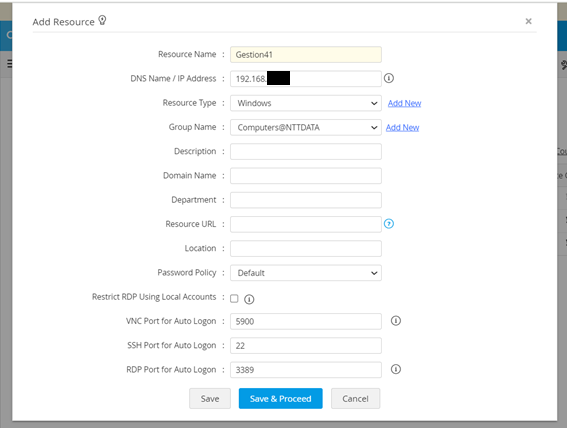
\includegraphics[width=0.8\textwidth]{./img/gestion41_importar.png}
	\caption{Gestión de contraseñas en PAM360.}
	\label{fig:gestion41_importar}
\end{figure}

\section{Gestión de contraseñas y acceso}
PAM360 se utilizó para gestionar contraseñas y controlar el acceso a diferentes recursos. La herramienta permitió la configuración de políticas de contraseñas y la asignación de roles a los usuarios. Esto aseguró que solo los usuarios autorizados pudieran acceder a ciertos recursos.

\begin{figure}[H]
	\centering
	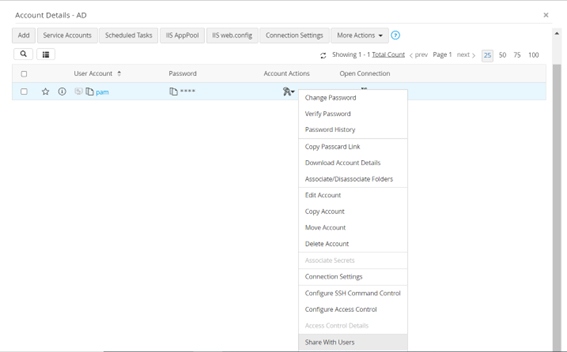
\includegraphics[width=0.8\textwidth]{./img/share_account_pam.png}
	\caption{Gestión de contraseñas en PAM360.}
	\label{fig:share_account_pam}
\end{figure}

Para conceder accesos en PAM es sencillo, se elige la cuenta de la máquina, la cual se va a ceder a un usuario. Seleccionamos la opción de "Share with Users".
Después, seleccionamos al usuario que le queremos dar acceso (en este caso, mi usuario)

\begin{figure}[H]
	\centering
	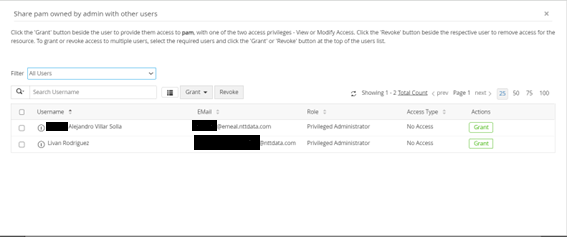
\includegraphics[width=0.8\textwidth]{./img/share_account_seleccion.png}
	\caption{Selección de usuario.}
	\label{fig:share_account}
\end{figure}

y seleccionamos la opción que deseemos, que sólo se pueda conectar a la máquina, que se pueda conectar y ver contraseñas o que pueda hacer todo incluso modificar contraseñas. Esta opciones varían dependiendo del tipo de privilegios que se le hayan concedido al usuario en PAM.

\begin{figure}[H]
	\centering
	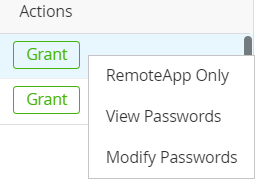
\includegraphics[width=0.8\textwidth]{./img/share-detail.png}
	\caption{Selección de usuario.}
	\label{fig:share_detail}
\end{figure}


Cuando tengamos contraseñas de máquinas guardadas y contraseñas asignadas, la portada de PAM cambiará y nos mostrará la información de nuestros sistemas

\begin{figure}[H]
	\centering
	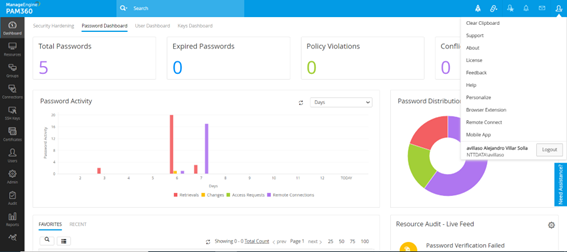
\includegraphics[width=0.8\textwidth]{./img/pam_portada_contodo.png}
	\caption{Configuración del administrador en PAM360.}
	\label{fig:pam_portadaactualizada}
\end{figure}

\section{Monitorización y auditoría}
Una vez configurado, PAM360 proporcionó capacidades de monitorización y auditoría que permitieron registrar todas las actividades de los usuarios. Esta funcionalidad es esencial para mantener la seguridad y cumplir con las políticas de la empresa.

El usuario accedería a la máquina a la cual tiene permiso. Introduciendo su usuario personal, tendría acceso a la máquina (en este caso Gestion42) como pam-access (cuenta la cual se ha creado para el uso de las máquinas). 

\begin{figure}[H]
	\centering
	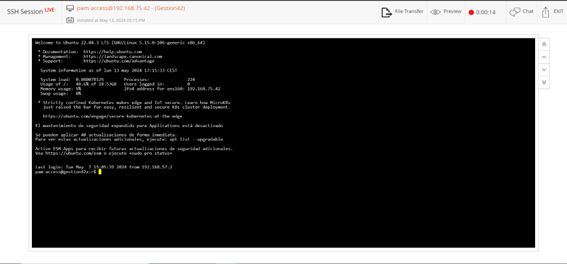
\includegraphics[width=0.8\textwidth]{./img/pam-ssh_live.png}
	\caption{Monitorización de actividades en PAM360.}
	\label{fig:pam_live}
\end{figure}

\begin{figure}[H]
	\centering
	\includegraphics[width=0.8\textwidth]{./img/pam_live.png}
	\caption{PAM360 configurado y operando.}
	\label{fig:pam_live2}
\end{figure}



\section{Resultados y validación}
Finalmente, se validó el correcto funcionamiento de PAM360 mediante pruebas exhaustivas. Dichas pruebas consistieron en mi tutor de la empresa y yo, cambiándonos los roles uno a otro, haciendo modificaciones en la máquina y el otro reportando dichas modificaciones para ver si se habían grabado correctamente. También se sometió a pruebas de penetración con Nessus y búsqueda de CVEs para PAM360, para comprobar si existía alguna vulnerabilidad. Se verificó que todos los usuarios importados pudieran acceder a los recursos según las políticas establecidas y que todas las actividades fueran registradas adecuadamente.Las acciones del usuario se quedan guardadas. Al acabar la sesión de uso pam proporciona reportes en modo de: PDF, html y vídeo.

También, el admin puede ver en tiempo real los movimientos que realizan los usuarios en las máquinas dentro de la propia solución.
\begin{figure}[H]
	\centering
	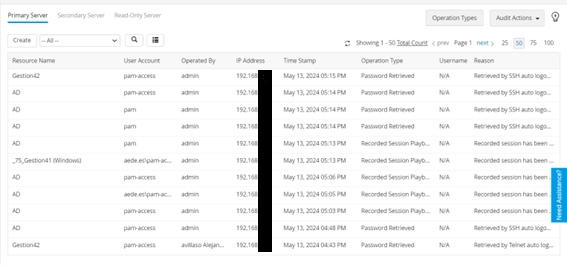
\includegraphics[width=0.8\textwidth]{./img/ad_movimientos.png}
	\caption{Monitorización de actividades en PAM360 en formato HTML.}
	\label{fig:ad_movimientos}
\end{figure}

Pero la información detallada sale al acabar la sesión
\begin{figure}[H]
	\centering
	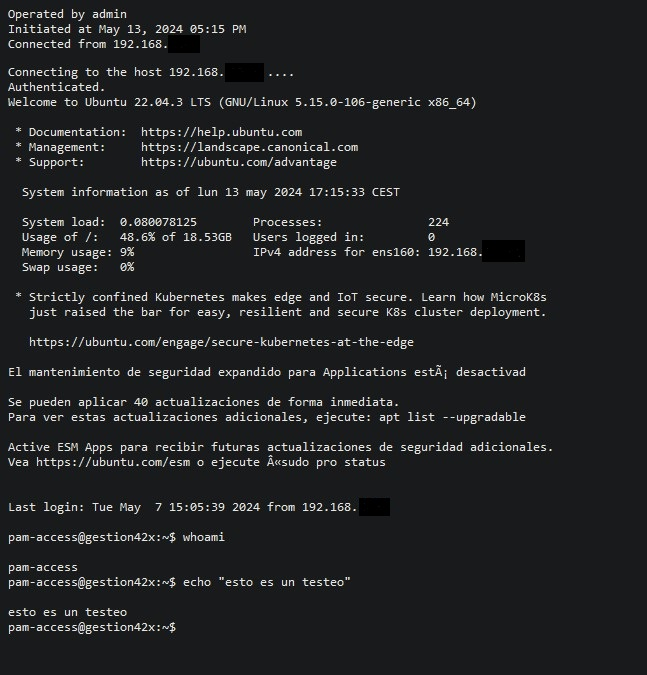
\includegraphics[width=0.8\textwidth]{./img/reporte_html.jpg}
	\caption{Resultados de la validación del sistema.}
	\label{fig:reporte_html}
\end{figure}




\capitulo{6}{Conclusiones y Líneas de trabajo futuras}

\section{Conclusiones}

Desarrollar el proyecto de implementación de PAM360 para NTT Data me ha proporcionado una visión clara de lo que esta herramienta puede hacer para mejorar la gestión de accesos privilegiados. Durante el proyecto, he conseguido cumplir con los principales objetivos, entre los cuales se destacan la mejora de la seguridad y la optimización de la gestión de accesos. A continuación, voy a detallar los objetivos alcanzados y las razones por las que considero que se han cumplido:

\begin{itemize}
	\item \textbf{Mejora de la seguridad:} Se ha implementado un control riguroso sobre el acceso a las máquinas, tanto para usuarios internos como para clientes. Esto ha reducido significativamente los riesgos de accesos no autorizados y ha añadido una capa extra de seguridad en la gestión de credenciales. Las capturas de pantalla que muestran el cambio de contraseña del administrador y la configuración de políticas de autenticación y recursos demuestran que se implementaron medidas de seguridad desde el inicio.
	
	\item \textbf{Optimización de la gestión de accesos:} PAM360 ha simplificado la administración de usuarios y contraseñas. Ya no es necesario crear cuentas específicas para cada máquina, lo que permite una gestión centralizada y mucho más eficiente, facilitando el trabajo de los administradores del sistema y mejorando la eficiencia operativa. Las imágenes capturadas del proceso de importación de usuarios desde Active Directory y la asignación de roles muestran cómo se centralizó la gestión de accesos.

	
	\item \textbf{Transparencia y trazabilidad:} Una de las grandes ventajas de PAM360 es su capacidad para registrar y auditar todas las actividades de los usuarios, asegurando así la transparencia y trazabilidad en el
	acceso a los recursos, lo cual es fundamental para cumplir con las normativas de seguridad y para las auditorías internas. Las imágenes de los reportes de auditoría y el dashboard de monitorización confirman la capacidad de PAM360 para registrar y auditar actividades.
	
	
	\item \textbf{Implementación técnica efectiva:} La instalación y configuración de PAM360 en un entorno virtualizado, utilizando herramientas como vSphere y MRemote, ha demostrado ser efectiva y robusta. Elegimos estas herramientas en la empresa porque facilitan el acceso y la administración remota del servidor PAM360. Las imágenes capturadas de la configuración de la máquina virtual en vSphere y del proceso de instalación de PAM360 evidencian una implementación técnica adecuada.

	
	\item \textbf{Integración con Active Directory:}La integración de PAM360 con el Active Directory de NTT Data ha permitido una sincronización fluida y efectiva de usuarios y roles, asegurando que los accesos se gestionen de manera centralizada y conforme a las políticas de la empresa. Las capturas que muestran la configuración del conector de Active Directory y la importación de usuarios evidencian
	una integración exitosa con AD.
	
	
	\item \textbf{Gestión segura de contraseñas:}La gestión de contraseñas con PAM360 ha sido intuitiva y segura, y la capacidad de generar reportes y auditorías ha sido especialmente útil para monitorizar y controlar los accesos en tiempo real. Las Instantáneas de pantalla de la configuración de políticas de contraseñas y los reportes de actividades demuestran la eficacia en la gestión segura de contraseñas y monitorización de accesos.  

\end{itemize}

\section{Líneas de Trabajo Futuras}

Sería recomendable ampliar el uso de PAM360 a todos los departamentos dentro de NTT Data, incluyendo la integración de todos los sistemas críticos bajo la gestión de PAM360, incrementando así su alcance y los beneficios que ofrece. Además, es importante explorar la automatización de tareas repetitivas y críticas utilizando las capacidades de scripting y API de PAM360. Esto no solo mejoraría la eficiencia operativa, sino que también reduciría el riesgo de errores humanos en la gestión de accesos.

Mantener una evaluación continua de las políticas de seguridad y las configuraciones de PAM360 es crucial para adaptarse a nuevas amenazas y vulnerabilidades. Actualizar estas políticas constantemente garantizará que la empresa se mantenga protegida contra posibles ataques. Finalmente, implementar programas de formación y capacitación para el personal técnico y administrativo de NTT Data sobre el uso y administración de PAM360 es fundamental. Una mejor comprensión y manejo de la herramienta contribuirán a maximizar su eficacia y a asegurar que todos los usuarios sigan las mejores prácticas de seguridad.

En resumen, el proyecto ha cumplido con sus objetivos iniciales y ha demostrado ser una solución efectiva para la gestión de accesos privilegiados en NTT Data. Las líneas de trabajo futuras propuestas permitirán no solo mantener, sino también mejorar y expandir las capacidades de seguridad y gestión de accesos en la empresa.



\bibliographystyle{plain}
\bibliography{C:/Users/darck/Desktop/TFG/plantillaLatex-master/bibliografia}



\end{document}
